\documentclass[10pt]{beamer}
\usetheme{metropolis}
\usepackage{amsmath, amssymb}
\usepackage{mathpartir}
\usepackage{listings}
\usepackage{xcolor}
\usepackage{tikz}

\definecolor{codegreen}{rgb}{0,0.6,0}
\definecolor{codegray}{rgb}{0.5,0.5,0.5}
\definecolor{codepurple}{rgb}{0.58,0,0.82}

\lstdefinestyle{lambdacalc}{
    basicstyle=\ttfamily\footnotesize,
    keywordstyle=\color{blue},
    commentstyle=\color{codegreen},
    numberstyle=\tiny\color{codegray},
    stringstyle=\color{codepurple},
    breakatwhitespace=false,         
    breaklines=true,                 
    keepspaces=true,                 
    numbers=left,       
    numbersep=5pt,                  
    showspaces=false,                
    showstringspaces=false,
    showtabs=false,                  
    tabsize=2,
    morekeywords={lambda, beta, eta, alpha, conv}
}

\title{Church-Rosser Theorems}
\subtitle{Confluence in Lambda Calculus}
\author{Amirreza Khakpour}
\date{September, 2025}

\begin{document}

\begin{frame}
\titlepage
\end{frame}

\begin{frame}{A Bit of History}
\begin{itemize}
\item Developed by Alonzo Church and his student J. Barkley Rosser in the 1930s
\item Part of the foundations of computability theory and functional programming
\item Lambda calculus emerged as an alternative to Turing machines for formalizing computation
\item Church-Rosser theorems establish fundamental properties about reduction strategies
\end{itemize}
\end{frame}

\begin{frame}{What is Lambda Calculus?}
A formal system for expressing computation using:
\begin{itemize}
\item \textbf{Variables}: \(x, y, z, \ldots\)
\item \textbf{Abstraction}: \(\lambda x.M\) (function creation)
\item \textbf{Application}: \(M\ N\) (function application)
\end{itemize}

\vspace{0.3cm}
\textbf{Examples}:
\begin{itemize}
\item Identity function: \(\lambda x.x\)
\item Constant function: \(\lambda x.\lambda y.x\)
\item Function application: \((\lambda x.x)\ y\)
\end{itemize}
\end{frame}

\begin{frame}{Lambda Calculus Syntax (Formally)}
\begin{align*}
M, N ::= &\ x \quad \text{(variable)} \\
\mid &\ \lambda x.M \quad \text{(abstraction)} \\
\mid &\ M\ N \quad \text{(application)}
\end{align*}

\textbf{Parentheses convention}: Application associates to the left
\[
M\ N\ P = (M\ N)\ P
\]

\textbf{Example}: \(\lambda f.\lambda x.f\ (f\ x)\) means \(\lambda f.(\lambda x.(f\ (f\ x)))\)
\end{frame}

\begin{frame}{Free and Bound Variables}
\begin{itemize}
\item \textbf{Bound variable}: Occurs in the body of a lambda abstraction
\item \textbf{Free variable}: Not bound by any enclosing lambda
\end{itemize}

\vspace{0.3cm}
\textbf{Example}: In \(\lambda x.x\ y\)
\begin{itemize}
\item \(x\) is bound (by \(\lambda x\))
\item \(y\) is free
\end{itemize}

\vspace{0.3cm}
\textbf{Alpha conversion}: Renaming bound variables
\[
\lambda x.x \equiv \lambda y.y
\]
\end{frame}

\begin{frame}{Beta Reduction (\(\beta\)-reduction)}
The main computational rule: function application
\[
(\lambda x.M)\ N \rightarrow_\beta M[x := N]
\]
where \(M[x := N]\) means substitute \(N\) for all free occurrences of \(x\) in \(M\).

\vspace{0.3cm}
\textbf{Example}:
\[
(\lambda x.x\ x)\ y \rightarrow_\beta y\ y
\]
\[
(\lambda x.\lambda y.x)\ z \rightarrow_\beta \lambda y.z
\]
\end{frame}

\begin{frame}{The Omega Combinator: Infinite Reduction!}
Consider this fascinating term:
\[
\Omega = (\lambda x.x\ x)(\lambda x.x\ x)
\]

Let's reduce it:
\[
\Omega \rightarrow_\beta (\lambda x.x\ x)(\lambda x.x\ x) \rightarrow_\beta (\lambda x.x\ x)(\lambda x.x\ x) \rightarrow_\beta \cdots
\]

\vspace{0.3cm}
\textbf{This reduces forever!} No normal form exists.

\vspace{0.3cm}
\textbf{Intuition}: A function that applies itself to itself, creating an infinite loop.
\end{frame}

\begin{frame}{More Non-Terminating Examples}
\begin{itemize}
\item \textbf{Omega combinator}: \(\Omega = (\lambda x.x\ x)(\lambda x.x\ x)\)
\item \textbf{Y combinator} (fixed-point combinator):
\[
Y = \lambda f.(\lambda x.f\ (x\ x))(\lambda x.f\ (x\ x))
\]
\item \textbf{Application to itself}: \(\lambda x.x\ x\)
\end{itemize}

\vspace{0.3cm}
\textbf{Crucial insight}: Some lambda terms have normal forms, some don't - just like some programs halt and some don't!
\end{frame}

\begin{frame}{Eta Reduction (\(\eta\)-reduction)}
Eliminates redundant abstractions:
\[
\lambda x.M\ x \rightarrow_\eta M \quad \text{(if \(x\) not free in \(M\))}
\]

\vspace{0.3cm}
\textbf{Example}:
\[
\lambda x.(\lambda y.y)\ x \rightarrow_\eta \lambda y.y
\]

\vspace{0.3cm}
\textbf{Intuition}: Two functions are extensionally equal if they produce the same output for all inputs.
\end{frame}

\begin{frame}{Reduction Strategies}
\begin{itemize}
\item \textbf{Normal order}: Reduce leftmost outermost redex first
\item \textbf{Applicative order}: Reduce leftmost innermost redex first
\item \textbf{Full reduction}: Reduce any redex in any order
\end{itemize}

\vspace{0.3cm}
\textbf{Crucial difference}: Normal order \textbf{will find} a normal form if one exists!

\vspace{0.3cm}
\textbf{Example}: \((\lambda x.\lambda y.y)(\Omega)\)
\begin{itemize}
\item Normal order: \(\rightarrow \lambda y.y\) (found normal form!)
\item Applicative order: Gets stuck reducing \(\Omega\) forever
\end{itemize}
\end{frame}

\begin{frame}{The Halting Problem Connection}
\begin{theorem}[Undecidability of Normal Form]
There is no algorithm that can decide, for an arbitrary lambda term \(M\), whether \(M\) has a normal form.
\end{theorem}

\vspace{0.3cm}
\textbf{This is equivalent to the Halting Problem!}

\vspace{0.3cm}
\textbf{Why?} We can encode Turing machines as lambda terms:
\begin{itemize}
\item Turing machine halts \(\Leftrightarrow\) corresponding lambda term has normal form
\item Reduction in lambda calculus \(\Leftrightarrow\) computation steps in Turing machine
\end{itemize}
\end{frame}

\begin{frame}{Original 1936 Paper Context}
\textbf{"Some Properties of Conversion" by Alonzo Church and J. Barkley Rosser}

\begin{itemize}
\item Published in Transactions of the American Mathematical Society, 1936
\item Uses original terminology: \textbf{conversion} (= reduction + expansion)
\item Defines: \(A \text{ conv } B\) means \(A\) and \(B\) are interconvertible
\item \textbf{Reduction}: Replacing a redex by its contractum
\item \textbf{Expansion}: Reverse of reduction
\end{itemize}
\end{frame}

\begin{frame}{Original Church-Rosser Theorems}
The 1936 paper contains three main theorems:

\begin{enumerate}
\item \textbf{Theorem 1}: Conversion sequencing theorem
\item \textbf{Theorem 2}: Normal form reachability theorem  
\item \textbf{Theorem 3}: Bound on reduction sequences theorem
\end{enumerate}

\vspace{0.3cm}
\textbf{Important}: These are more nuanced than the modern "diamond property" version!
\end{frame}

\begin{frame}{Theorem 1: Conversion Sequencing}
\begin{theorem}[Church-Rosser Theorem 1, 1936]
If \(A \text{ conv } B\), then there is a conversion from \(A\) to \(B\) in which no expansion precedes any reduction.
\end{theorem}

\vspace{0.3cm}
\textbf{Modern interpretation}: Any equivalence proof can be rearranged as:
\[
A \rightarrow^* C \leftarrow^* B
\]
where all reductions happen first, then all expansions.

\vspace{0.3cm}
\textbf{Significance}: Establishes that β-equivalence classes have a "diamond" structure.
\end{frame}

\begin{frame}{Theorem 1 Visualized}
\begin{center}
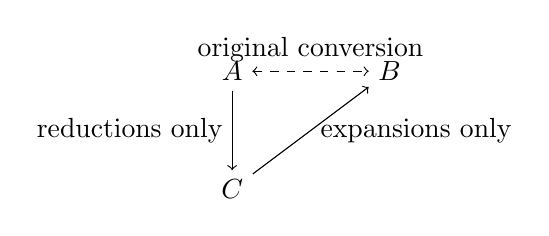
\begin{tikzpicture}[node distance=2cm]
\node (A) {\(A\)};
\node (B) [right of=A] {\(B\)};
\node (C) [below of=A, node distance=1.5cm] {\(C\)};

\draw[<->, dashed] (A) -- node[above] {original conversion} (B);
\draw[->] (A) -- node[left] {reductions only} (C);
\draw[<-] (B) -- node[right] {expansions only} (C);
\end{tikzpicture}
\end{center}

\textbf{Example}: If \(A \leftarrow X \rightarrow Y \leftarrow B\), then there exists \(C\) with \(A \rightarrow^* C \leftarrow^* B\).
\end{frame}

\begin{frame}{Theorem 2: Normal Form Reachability}
\begin{theorem}[Church-Rosser Theorem 2, 1936]
If \(B\) is a normal form of \(A\), then there is a number \(m\) such that any sequence of reductions from \(A\) will lead to \(B\) (to within applications of alpha conversion) after at most \(m\) reductions.
\end{theorem}

\vspace{0.3cm}
\textbf{Modern interpretation}: 
\begin{itemize}
\item If a normal form exists, it's reachable in bounded steps
\item All reduction sequences of sufficient length will find it
\item Accounts for alpha conversion (renaming bound variables)
\end{itemize}
\end{frame}

\begin{frame}{Theorem 2 Example}
Consider: \((\lambda x.x\ x)((\lambda y.y)\ z)\)

\begin{itemize}
\item Normal form: \(z\ z\)
\item Maximum needed reductions: 3
\item Any reduction sequence of length ≥ 3 will reach \(z\ z\) (up to alpha)
\end{itemize}

\vspace{0.3cm}
\textbf{Contrast with Ω}: \((\lambda x.x\ x)(\lambda x.x\ x)\) has no normal form, so no such \(m\) exists.
\end{frame}

\begin{frame}{Theorem 3: Bound on Reduction Sequences}
\begin{theorem}[Church-Rosser Theorem 3, 1936]
If \(A\) has a normal form, then there is a number \(m\) such that at most \(m\) reductions of order one can occur in a sequence of reductions on \(A\).
\end{theorem}

\vspace{0.3cm}
\textbf{Order one reduction}: Reducing a redex that is not contained in any other redex.

\vspace{0.3cm}
\textbf{Significance}: There's a finite bound on how many "top-level" reductions can occur, regardless of reduction strategy.
\end{frame}

\begin{frame}{Understanding "Order One" Reductions}
\textbf{Order one}: Outermost redexes not contained in other redexes.

\vspace{0.3cm}
\textbf{Example}: In \((\lambda x.x\ x)((\lambda y.y)\ z)\)
\begin{itemize}
\item Order one: \((\lambda x.x\ x)((\lambda y.y)\ z)\) itself
\item Not order one: \((\lambda y.y)\ z\) (contained in the larger redex)
\end{itemize}

\vspace{0.3cm}
\textbf{Theorem 3 says}: Only finitely many such top-level reductions possible if normal form exists.
\end{frame}

\begin{frame}{Normal Order Evaluation to the Rescue!}
\begin{theorem}[Standardization Theorem]
If a term has a normal form, normal order reduction will find it.
\end{theorem}

\vspace{0.3cm}
\textbf{Example}: \((\lambda x.\lambda y.y)(\Omega)\)
\begin{itemize}
\item Normal order: Reduces to \(\lambda y.y\) (success!)
\item Applicative order: Gets stuck reducing \(\Omega\) forever
\end{itemize}

\vspace{0.3cm}
\textbf{Practical significance}: This is why lazy evaluation (like in Haskell) can handle infinite data structures!
\end{frame}

\begin{frame}{Relationship to Modern Church-Rosser}
\begin{itemize}
\item \textbf{Modern version}: Usually stated as confluence: \(M \rightarrow^* N_1\) and \(M \rightarrow^* N_2\) implies exists \(P\) with \(N_1 \rightarrow^* P\) and \(N_2 \rightarrow^* P\)
\item \textbf{Original Theorem 1}: Stronger - deals with full conversion (reduction + expansion)
\item \textbf{Original Theorems 2 \& 3}: Provide quantitative bounds not in modern statements
\end{itemize}

\vspace{0.3cm}
\textbf{Historical note}: The "diamond property" proof came later and is often easier to work with.
\end{frame}

\begin{frame}{Proof Sketch (High Level)}
\begin{enumerate}
\item Define \textbf{parallel reduction}: Reduce multiple non-overlapping redexes simultaneously
\item Prove diamond property for parallel reduction
\item Show that the transitive closure of parallel reduction equals ordinary reduction
\item Conclude that ordinary reduction has the Church-Rosser property
\end{enumerate}

\vspace{0.3cm}
\textbf{Key insight}: By allowing parallel reductions, we avoid the "diamond problem" where reductions interfere with each other.
\end{frame}

\begin{frame}{Significance and Applications}
\begin{itemize}
\item \textbf{Functional programming}: Evaluation order doesn't affect final result (if it exists)
\item \textbf{Compiler optimization}: Freedom to rearrange computations
\item \textbf{Theorem proving}: Basis for rewriting systems and equality reasoning
\item \textbf{Programming language theory}: Foundation for many type systems
\item \textbf{Undecidability}: Shows fundamental limits of computation
\end{itemize}
\end{frame}

\begin{frame}{Summary: Key Takeaways}
\begin{itemize}
\item Lambda calculus provides a foundation for computation
\item Some terms have normal forms, some don't (like Ω)
\item Normal form existence is undecidable (equivalent to halting problem)
\item Original Church-Rosser theorems provide deep insights about conversion
\item Theorems 2 and 3 give quantitative bounds on reduction sequences
\item Normal order evaluation will find a normal form if one exists
\end{itemize}

\vspace{0.5cm}
\begin{center}
\textbf{Questions?}
\end{center}
\end{frame}

\end{document}